% Created 2023-09-28 Thu 12:45
% Intended LaTeX compiler: pdflatex
\documentclass[10pt,t]{article}
\usepackage[utf8]{inputenc}
\usepackage[T1]{fontenc}
\usepackage{graphicx}
\usepackage{longtable}
\usepackage{wrapfig}
\usepackage{rotating}
\usepackage[normalem]{ulem}
\usepackage{amsmath}
\usepackage{amssymb}
\usepackage{capt-of}
\usepackage{hyperref}
\author{Christopher Hepplewhite}
\date{\today}
\title{\large Evolution and Status of the Stand-Alone Radiative Transfer Algorithm (SARTA)}
\hypersetup{
 pdfauthor={Christopher Hepplewhite},
 pdftitle={\large Evolution and Status of the Stand-Alone Radiative Transfer Algorithm (SARTA)},
 pdfkeywords={},
 pdfsubject={},
 pdfcreator={Emacs 28.1 (Org mode 9.5.2)}, 
 pdflang={English}}
\begin{document}

\maketitle

\section{SAMPLE: Motivation}
\label{sec:orgd932b0f}
\begin{itemize}
\item Produce Level 1b AIRS,CrIS, IASI and CHIRP radiances for trending and retrievals.
\item Goals
\begin{itemize}
\item Radiometric stability, inter-sensor bias, intra-sampling bias and trending analysis.
\end{itemize}
\end{itemize}
\vspace{0.05in}

Working in radiance space is in principle very simple and quick.  Allows frequent re-processing. 

\vspace{0.05in}

What's Hard: 
\begin{itemize}
\item Dealing with clouds
\item AIRS radiometric stability estimates (ie. how good?)
\end{itemize}

\section{Outline of talk}
\label{sec:org9de1cb5}
\begin{itemize}
\item Historical Context
\item Design Features
\item Strengths
\item Limitations
\item Applications examples
\item Current Needs, Future Developments
\end{itemize}

\section{Historical Context}
\label{sec:org6c3d854}

\begin{itemize}
\item The SARTA was developed on 1990s computer systems - light load and memory requirements.
\item Origninaly developed as part of AIRS level 2 retrieval suite.
\item First supplied to AIRS project with separate coefficient sets for different instrument focal
plane and filter temperatures.
\item Since 2016 SARTA was delivered for the AIRS.L1C channel SRF specification.
\item Used for AIRS validation and more recently for CrIS and IASI validation.
\item In the past couple of years has been adapted for use with CHIRP.
\end{itemize}


\section{Attributes: Strengths}
\label{sec:org018d11a}
\begin{itemize}
\item Implicitly high speed computation (even more on modern systems).
\item SARTA is available for clear-sky and all-sky (scattering) computations.
\item Flexible channel selection, multi-sensor compatible, relatively quick development/update turn-around.
\item The scattering version uses a fast 2-slab model for clouds and aerosols (S. De Souza-Machado).
\item Model includes H2O, CO2, O3, N2O, CO, CH4, HNO3, HDO, SO2, NH3, nonLTE (4.3 um), Surface emissivity
and albedo, scattering from water, ice, aerosols, smoke.  Other absorbers could be added.
\item Accuracy well quantified.
\end{itemize}

\section{Attributes: Dependencies}
\label{sec:org795b3c5}
\begin{itemize}
\item Fast coefficients are derived using Optical Depths calculated using kCARTA - the pseudo-line by line
RTA (S. De Souza-Machado)
\item The atmospheric layering is currently defined as the 101 AIRS levels set, using Klayers algorithm.
\item The atmospheric layering can be changed (see later).
\item The data format for file I/O uses the HDF4 specification (original to AIRS project) (see later).
\item The spectral line shapes use the HITRAN databases, cross-sections and various dust and aerosol models.
\item Code is written in FORTRAN (this is NOT a limitation!).
\item Radiometric accuracy may be improved with tuning in some regions.
\end{itemize}

\section{Attributes: Limitations}
\label{sec:org40bf8bc}
\begin{itemize}
\item Finite diff Jacs - until now !
\item HDF4 dependency.
\end{itemize}

\section{Most Recent updates}
\label{sec:orgd1faf21}
\begin{itemize}
\item HITRAN 2020 spectroscopy (actual data available early 2022).
\item HDO included.
\item New nonLTE model being tested.
\end{itemize}


\section{Updates 1: HITRAN 2020 vs 2016}
\label{sec:org4e51110}
\begin{itemize}
\item Most significant change in 1050 cm-1 O3 band.
\end{itemize}
\begin{center}
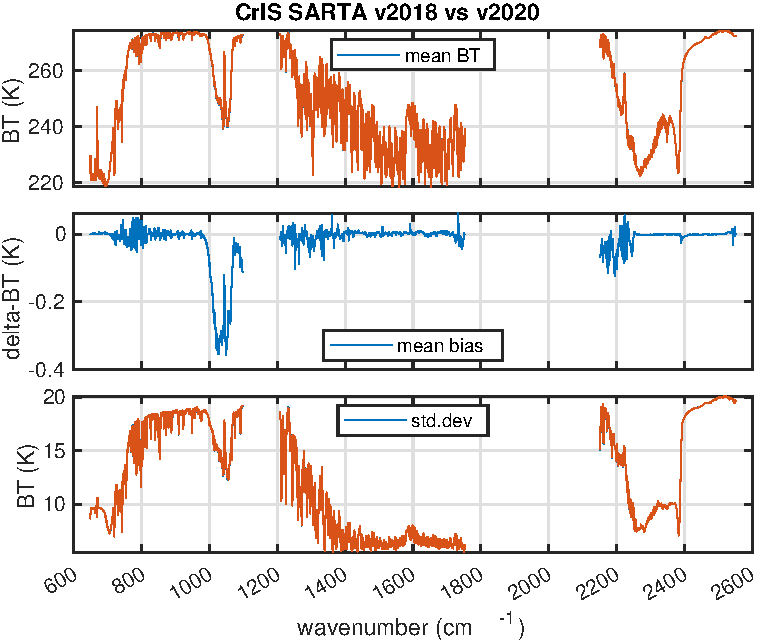
\includegraphics[width=.9\linewidth]{./Figs/sarta_cris_hr_h2018_vs_h2020_r49_686_mn_stdaslp.pdf}
\end{center}

\section{Updates 2: HDO included}
\label{sec:orgba4c83e}

\section{Updates 3: nonLTE}
\label{sec:org2f6bb28}

\section{Beneficial Future Changes}
\label{sec:org28582a2}
\begin{itemize}
\item Make independent (agnostic) of file format types (HDF4, H5, netCDF).
\item Simplify packaging and coefficient management.
\item Extend/update training set, add machine learning if demonstrably beneficial.
\item Adapt to the cloud and complete open-source migration (documentation).
\item Re-package code with Julia or Python wrappers for wider community use.
\item Include as part of CHIRP processing suite (cloud).
\end{itemize}

\section{Future 1: File format, Coefficient packaging}
\label{sec:orgc21da4f}

\section{Future 2: Adapt to Cloud}
\label{sec:orgf169979}
\end{document}